\documentclass[12pt, a4paper]{article}
\usepackage{ctex}
\usepackage{graphicx}
\usepackage{float}
\usepackage[super, square]{natbib}
\usepackage{booktabs}
\usepackage[margin = 1in]{geometry}
\usepackage{
  color,
  clrscode,
  amssymb,
  ntheorem,
  amsmath,
  listings,
  fontspec,
  xcolor,
  supertabular,
  multirow
}
\renewcommand\contentsname{Contents}
\renewcommand\refname{References}
\renewcommand\figurename{Fig.}
\definecolor{bgGray}{RGB}{36, 36, 36}
\usepackage[
  colorlinks,
  linkcolor=bgGray,
  anchorcolor=blue,
  citecolor=black
]{hyperref}
\newfontfamily\courier{Courier New}

\theoremstyle{margin}
\theorembodyfont{\normalfont}

\newtheorem{theorem}{Theorem}
\newtheorem{definition}[theorem]{Definition}
\newtheorem{example}[theorem]{Example}

\newcommand{\st}{\text{s.t.}}
\newcommand{\mn}{\mathnormal}
\newcommand{\tbf}{\textbf}
\newcommand{\fl}{\mathnormal{fl}}
\newcommand{\f}{\mathnormal{f}}
\newcommand{\g}{\mathnormal{g}}
\newcommand{\R}{\mathbf{R}}
\newcommand{\Q}{\mathbf{Q}}
\newcommand{\JD}{\textbf{D}}
\newcommand{\rd}{\mathrm{d}}
\newcommand{\str}{^*}
\newcommand{\vep}{\varepsilon}
\newcommand{\lhs}{\text{L.H.S}}
\newcommand{\rhs}{\text{R.H.S}}
\newcommand{\con}{\text{Const}}
\newcommand{\oneton}{1,\,2,\,\dots,\,n}
\newcommand{\aoneton}{a_1a_2\dots a_n}
\newcommand{\xoneton}{x_1,\,x_2,\,\dots,\,x_n}

\title{Project Report of RISC-V CPU}
\author{Weizhe Chen (陈伟哲)\\ACM Class, Shanghai Jiao Tong University}
\date{}

\begin{document}

\lstset{numbers=left,
  basicstyle=\scriptsize\courier,
  numberstyle=\tiny\courier\color{red!89!green!36!blue!36},
  language=C++,
  breaklines=true,
  keywordstyle=\color{blue!70},commentstyle=\color{red!50!green!50!blue!50},
  morekeywords={},
  stringstyle=\color{purple},
  frame=shadowbox,
  rulesepcolor=\color{red!20!green!20!blue!20}
}
\maketitle

\section{Introduction}

This project is a RISC-V CPU with five-stage pipeline, implemented in Verilog HDL.

\section{Design}

\subsection{Features}

Main features of this RISC-V CPU are briefly introduced in the table below.

\begin{table}[H]
\centering
\begin{tabular}{@{}ll@{}}
\toprule
\multicolumn{1}{c}{Feature} & \multicolumn{1}{c}{RISC-V CPU}                                                                        \\ \midrule
ISA                         & RISC-V(subset) \\
Cache                       & 2-way set associate I-cache\\
Branch Prediction           & static branch prediction which always predict not jump\\
FPGA Support                & Yes\\
Speed                       & 100Mhz 1.6s for pi.c*\\
 \bottomrule
\end{tabular}
\end{table}

[*]: When running 100Mhz on FPGA, it has timing failed problem , but it still run pretty good.

\iffalse

\begin{table}[H]
\centering
\begin{tabular}{@{}ll@{}}
\toprule
\multicolumn{1}{c}{Speed} & \multicolumn{1}{c}{RISC-V CPU}                                                                        \\ \midrule
ISA                         & RISC-V(subset) \\
Cache                       & 2-way set associate I-cache\\
Branch Prediction           & static branch prediction which always predict not jump\\
FPGA Support                & Yes\\
 \bottomrule
\end{tabular}
\end{table}

\fi

\subsection{Specification}

My CPU is a standard 5-stage pipeline CPU which has a memory controller and stall controller. It also have a I-cache  and a static branch prediction for speed up.

\begin{itemize}
\item Considering all hazards. For structure hazard, we don't need to face it. For data hazard, I used the forwarding method to solve it. But when facing with LOAD command which I can not get the exactly value of register before MEM stage, I have to stall the pipeline until the former command pass MEM stage. For control hazard, when I found there is a branch prediction fault, I just changed those commands into no-use commands which is actually bubbles.

\begin{figure}[H]
	\begin{center}
	  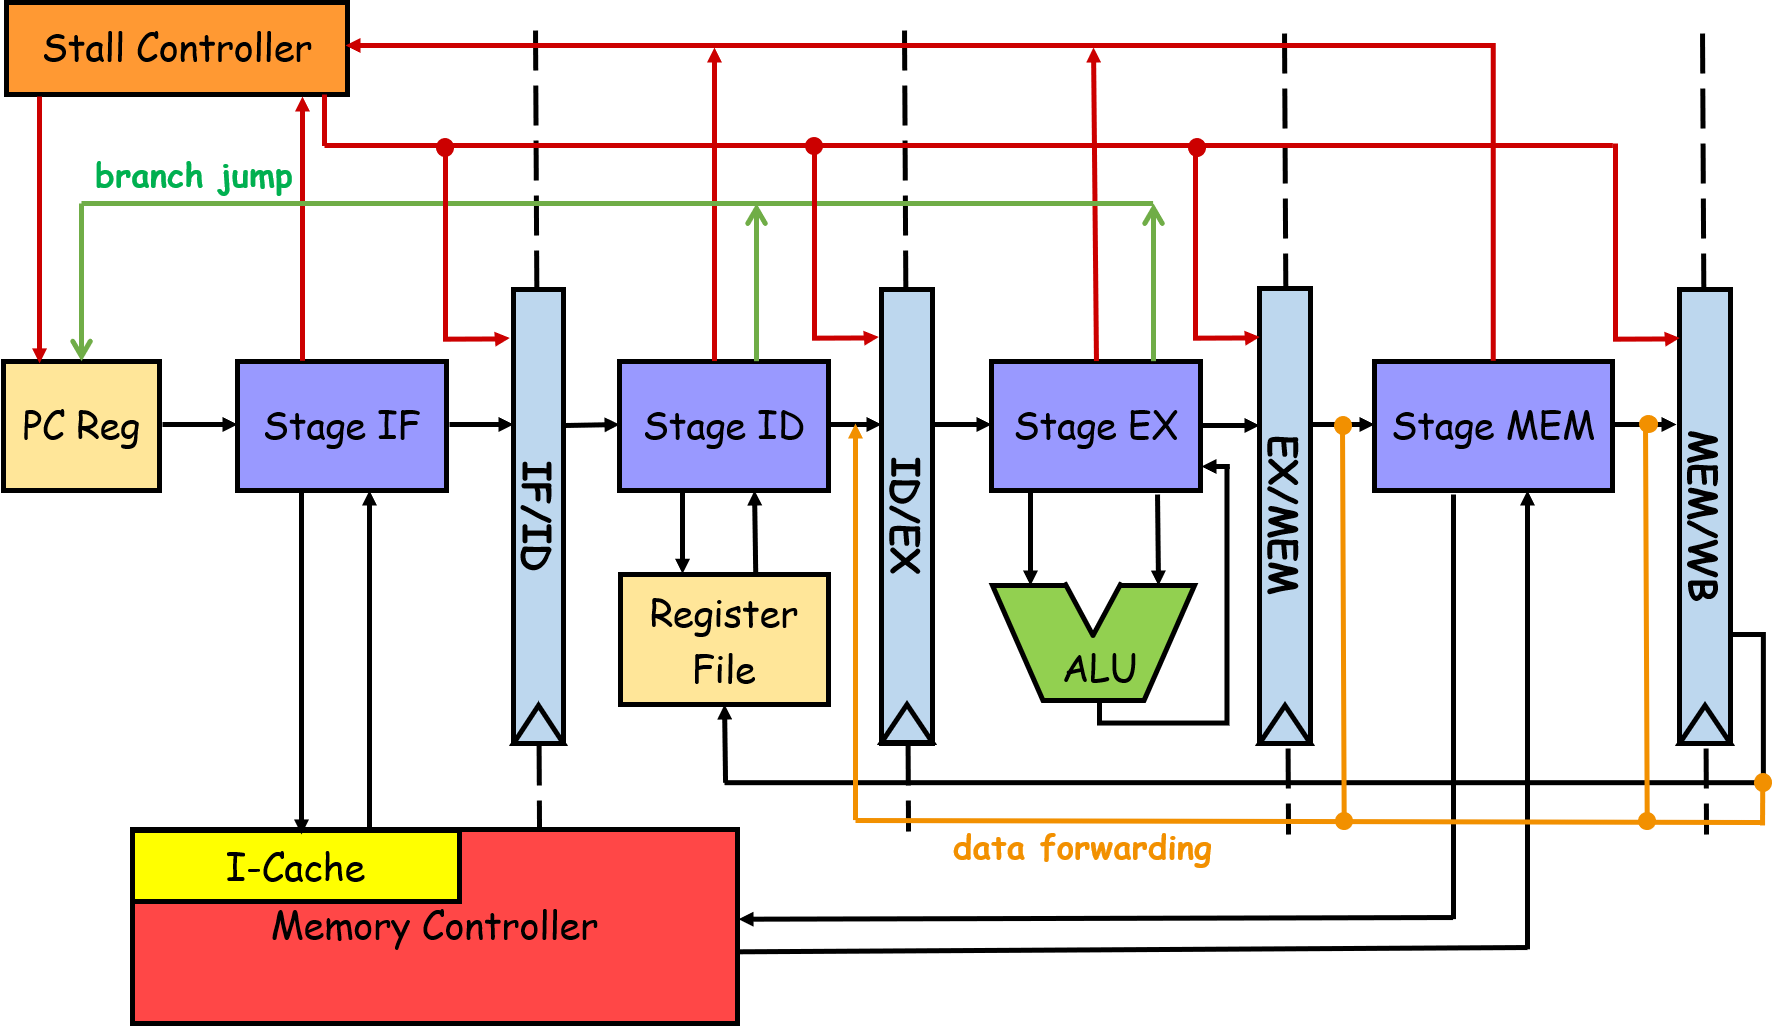
\includegraphics[height=9cm]{structure.png}
	\end{center}
	\caption{Structure of my CPU Design}
\end{figure}


%	\item Because of the limit that we can only get 1 byte a time, the CPU often need to be stalled when Instruction need to be fetched or the CPU meet a LOAD/STORE instruction.That envolves a stall control module which helps to control the pipeline to ensure it works well.



    \item Although facing with timing failed for 100Mhz in my implementation period, I can run the CPU correctly on the FPGA. The biggest reason is that almost all the timing failed is because I have a module using negedge in the CPU, which makes it has less time permitted. I use it in the part that I-cache updating and it should be done before the next posedge otherwise if the new pc is equal to the former pc, it can not hit. It can be fixed by a few code rewriting ( actually special check for this case).
\end{itemize}

\section{Thinkings about features}

\paragraph{Cache} Cache is urgently needed  because the speed of communication with memory is really the bottleneck of this CPU. One simple instruction to be fetched need 4 cycle without cache. And with no write on instruction memory, a I-cache is a choice that is not only easy to write but also useful. My I-cache is a 2-way set associate cache, with LRU method when facing replacing problem.The cache size is 2K.

\paragraph{Branch Prediction} A static prediction is used in my CPU. And it will always predict not jump. The reason for a prediction like that is that it don't need extra calculation because $pc_{new} = pc_{current} + 4$ is already calculated even before we know it is a branch command.For any other branch prediction method, we have to flush the pipeline because the next pc is already readed when we do the prediction. We may add a BTB in fetch stage, but it does not work very well according to some of my classmates sayings.

\section{Acknowledgements}
Special thanks to Linqi Chen (陈林淇) for his guidance to me of how to use Vivado and a few suggestions of writing which truly helpes me to run on the FPGA. Also thanks many other classmates for their suggestions and help.

\section{References}
\iffalse
\begin{thebibliography}{9}
  \bibitem{lsl}
  	雷思磊.
  	\emph{自己动手写CPU},
  	电子工业出版社, 2014.
  \bibitem{wzh}
  	Zhanghao Wu's (吴章昊) MIPS CPU project.
  	\url{https://github.com/Michaelvll/RISCV_CPU}

\end{thebibliography}
\fi

\begin{enumerate}
    \item [1.]雷思磊.\emph{自己动手写CPU},电子工业出版社, 2014.
    \item [2.]Zhanghao Wu's (吴章昊) MIPS CPU project.
  	\url{https://github.com/Michaelvll/RISCV_CPU}
\end{enumerate}

\end{document}
